\documentclass[aspectratio=169]{beamer}

% Theme Configuration
\usetheme{Madrid}
\useoutertheme{miniframes}
\usecolortheme{seahorse}

% Packages
\usepackage{graphicx}
\usepackage{amsmath}
\usepackage{animate} % For embedded frame-by-frame animations
\usepackage{booktabs}
\usepackage{hyperref}

% Robust path searching for Overleaf uploads
\graphicspath{{images/}{ppt_image/}{images/ppt_image/}{./}}

% Title Information
\title[Surrogate Modeling \& Active Learning]{Surrogate Modeling and Active Learning for Collision-Avoidance Crowd Dynamics}
\subtitle{From Microscopic Langevin Dynamics to Data-Driven Emulation}
\author[S. K. Gupta]{Saurabh Kumar Gupta}
\institute[NIT Mizoram \& KIT]{
    Supervisors: Emil Loevbak, Prof. Dr. Martin Frank \\
    \vspace{0.3cm}
    National Institute of Technology (NIT) Mizoram, India \\
    Karlsruhe Institute of Technology (KIT), SCC, Germany
}
\date{July 30, 2026}

\begin{document}

% ----------------------------------------------------
% Slide 1: Title Slide
% ----------------------------------------------------
\begin{frame}
    \titlepage
\end{frame}

% ----------------------------------------------------
% Section 1: Introduction, Motivation & Physics
% ----------------------------------------------------
\section{Physics Foundations}

\begin{frame}{Microscopic Foundations of Crowd Dynamics}
    \textbf{Traditional Social Force Model (SFM)}
    \vspace{0.2cm}
    
    Treats crowd movement as nonlinearly coupled Langevin differential equations. Pedestrian $i$ balances a driving force $\vec{f}_{i}^{0}$ and exponential psychological/physical repulsion forces $\vec{f}_{ij}$.
    
    \begin{block}{SFM Governing Equations}
    \[
    \vec{f}_{i}^{0} = m_{i}\frac{\vec{v_{i}^{0}}(t)\vec{e_{i}}(t)-\vec{v_{i}}(t)}{\tau_{i}} 
    \]
    \[
    \vec{f}_{ij}^{psy} = A_{i}\exp[(r_{ij}-d_{ij})/B_{i}]\vec{n}_{ij}
    \]
    \end{block}

    \vspace{0.3cm}
    \textbf{\textcolor{red}{The Flaw:}} Classic SFM relies on massive contact forces ($K = 120,000$ N/m) and psychological repulsion ($A = 2000$ N). It lacks an anticipatory steering radar, causing artificial gridlocks in high-density counterflow.
\end{frame}

\begin{frame}{Collision-Avoidance Force Model (CAFM)}
    \textbf{Proactive Spatial Anticipation} (Yang et al. 2024)
    \vspace{0.2cm}

    Introduces the Bird-oid Objects (BOIDS) autonomous steering algorithm to model active pedestrian collision avoidance using a forward-facing radar.
    
    \begin{itemize}
        \item Safety vector $\vec{R}_{safety}$ and a danger threshold $\vec{R}_{danger} = 0.5 \times \vec{R}_{safety}$.
        \item \textbf{Avoidance Force ($\vec{f}_{ad}$):} Triggered when distance $d$ falls within radar ($r < d < R$).
    \end{itemize}

    \begin{block}{Avoidance Vector}
    \[
    \vec{f}_{ad}=\frac{\vec{R}_{safety-obstacle}}{|\vec{R}_{safety-obstacle}|}f_{adm}
    \]
    \end{block}

    \textbf{Empirical Calibration:} Calibrated via UAV drone footage. Maximum force $f_{adm} = 38,800$ N, safety range $R_{safety} = 1.22$ m. This slashes the classical psychological noise $A$ down from 2000 to just 20.
\end{frame}

\begin{frame}{Visualizing the CAFM Dynamics}
    \begin{center}
        % Make sure cafm_simulation.gif exists in the same folder
        \animategraphics[autoplay,loop,width=0.7\textwidth]{7}{cafm_frames_fast/frame_}{0}{49}
    \end{center}
    
    \vspace{0.2cm}
    \begin{itemize}
        \item \textbf{Observation:} Pedestrians utilize predictive avoidance forces to naturally form smooth, bi-directional lanes, preventing the gridlock seen in classic SFM.
    \end{itemize}
\end{frame}

\begin{frame}{The Computational Bottleneck}
    \begin{itemize}
        \item \textbf{The Curse of Dimensionality:} Simulating emergency dynamics or finding crowd phase-transitions requires searching a continuous 6-dimensional parameter space.
        \item \textbf{HPC Constraint:} Numerically integrating millions of microscopic Langevin ODE timesteps for systematic Uncertainty Quantification (UQ) is computationally prohibitive.
    \end{itemize}

    \vspace{0.4cm}
    \begin{alertblock}{Project Objectives}
        \begin{enumerate}
            \item Build a fast, data-driven machine learning \textbf{Surrogate Model} to act as a black-box emulator.
            \item Achieve high generalization accuracy mapping 6 inputs to 4 macroscopic metrics using a strict budget of only 256 initial simulation training blocks.
        \end{enumerate}
    \end{alertblock}
\end{frame}

% ----------------------------------------------------
% Section 2: Data Engineering
% ----------------------------------------------------
\section{Data Engineering}

\begin{frame}{Parameter Spaces \& Design of Experiments (DoE)}
    \textbf{The 6D Input Vector ($\mathbf{x}$):} Swept across behavioral and environmental boundaries:
    \begin{itemize}
        \item \texttt{v0\_mean}: $[0.80, 1.60]$ m/s \quad \texttt{tau}: $[0.30, 0.80]$ s
        \item \texttt{A}: $[10.0, 40.0]$ N \quad \texttt{R\_safety}: $[0.80, 1.60]$ m
        \item \texttt{density}: $[0.10, 1.00]$ agents/m$^2$ \quad \texttt{flow\_ratio}: $[0.00, 0.50]$
    \end{itemize}

    \textbf{The 4D Output Vector ($\mathbf{y}$):}
    \begin{itemize}
        \item \texttt{mean\_crossing\_time}, \texttt{flow\_rate}, \texttt{order\_param\_mean}, \texttt{mean\_speed}
    \end{itemize}

    \vspace{0.3cm}
    \textbf{DoE Evolution:} Upgraded from classic Latin Hypercube Sampling (LHS) to low-discrepancy \textbf{Quasi-Monte Carlo (QMC) Sobol Sequences} to guarantee optimal space-filling properties.
\end{frame}

\begin{frame}{Automated HPC Simulation Pipeline}
    \begin{itemize}
        \item Coded a modular, reproducible pipeline matching the geometry of Yang et al.'s outdoor experiment (26 m $\times$ 3 m corridor with a central 10 m measurement window).
        \item \textbf{Aleatoric Noise Mitigation:} Pedestrian systems exhibit stochastic micro-chaos (random seed variations).
    \end{itemize}

    \vspace{0.4cm}
    \begin{block}{Batch Pipeline Processing}
        The script executed the 256 Sobol points with 3 parallel randomized repeats per point, averaging the output tensors to extract the true underlying physics into \texttt{cafm\_qmc\_256.npz}.
    \end{block}
\end{frame}

% ----------------------------------------------------
% Section 3: Surrogate Architecture
% ----------------------------------------------------
\section{Surrogate Architecture}

\begin{frame}{Heteroscedastic Gaussian Processes}
    \textbf{Why avoid deep neural networks?} They output deterministic point-predictions. Safety-critical systems require well-calibrated epistemic uncertainty estimates ($\sigma^2$).

    \vspace{0.2cm}
    \textbf{Gaussian Process Regression (GPR):} Defines a non-parametric Bayesian prior over continuous functions: $f(\mathbf{x}) \sim \mathcal{GP}(m(\mathbf{x}), k(\mathbf{x}, \mathbf{x}'))$.

    \vspace{0.2cm}
    We engineered independent parallel prediction matrices. Rather than assuming uniform global noise, we inject the empirical simulation variance floor ($\mathbf{V}_{i,t}$) directly into the marginal log-likelihood inversion:

    \begin{block}{Log-Likelihood}
    \[
    \log p(\mathbf{y} \mid \mathbf{X}) = -\frac{1}{2}\mathbf{y}^T(\mathbf{K} + \mathbf{V})^{-1}\mathbf{y} - \frac{1}{2}\log\det(\mathbf{K} + \mathbf{V}) - \frac{N}{2}\log(2\pi)
    \]
    \end{block}
\end{frame}

\begin{frame}{Covariance Mechanics \& Dimension Reduction}
    \textbf{The Matérn $\nu=2.5$ Kernel:} Restricts functions to $C^2$ differentiability. This allows the surrogate to perfectly track sudden physical phase-changes (free-flow to gridlock) without the unphysical numerical "ringing" artifacts of RBF kernels.

    \vspace{0.3cm}
    \textbf{Automatic Relevance Determination (ARD):} Operates as an implicit feature selector by optimizing a separate length-scale ($l_i$) for each of the 6 dimensions:

    \begin{block}{ARD Kernel Distance}
    \[
    d^2(\mathbf{x}, \mathbf{x}') = \sum_{i=1}^{6} \frac{(x_i - x'_i)^2}{l_i^2}
    \]
    \end{block}
    \textit{Large $l_i$ implies the output is insensitive to that dimension.}
\end{frame}

\begin{frame}{Automatic Relevance Determination (ARD) Results}
    \begin{center}
        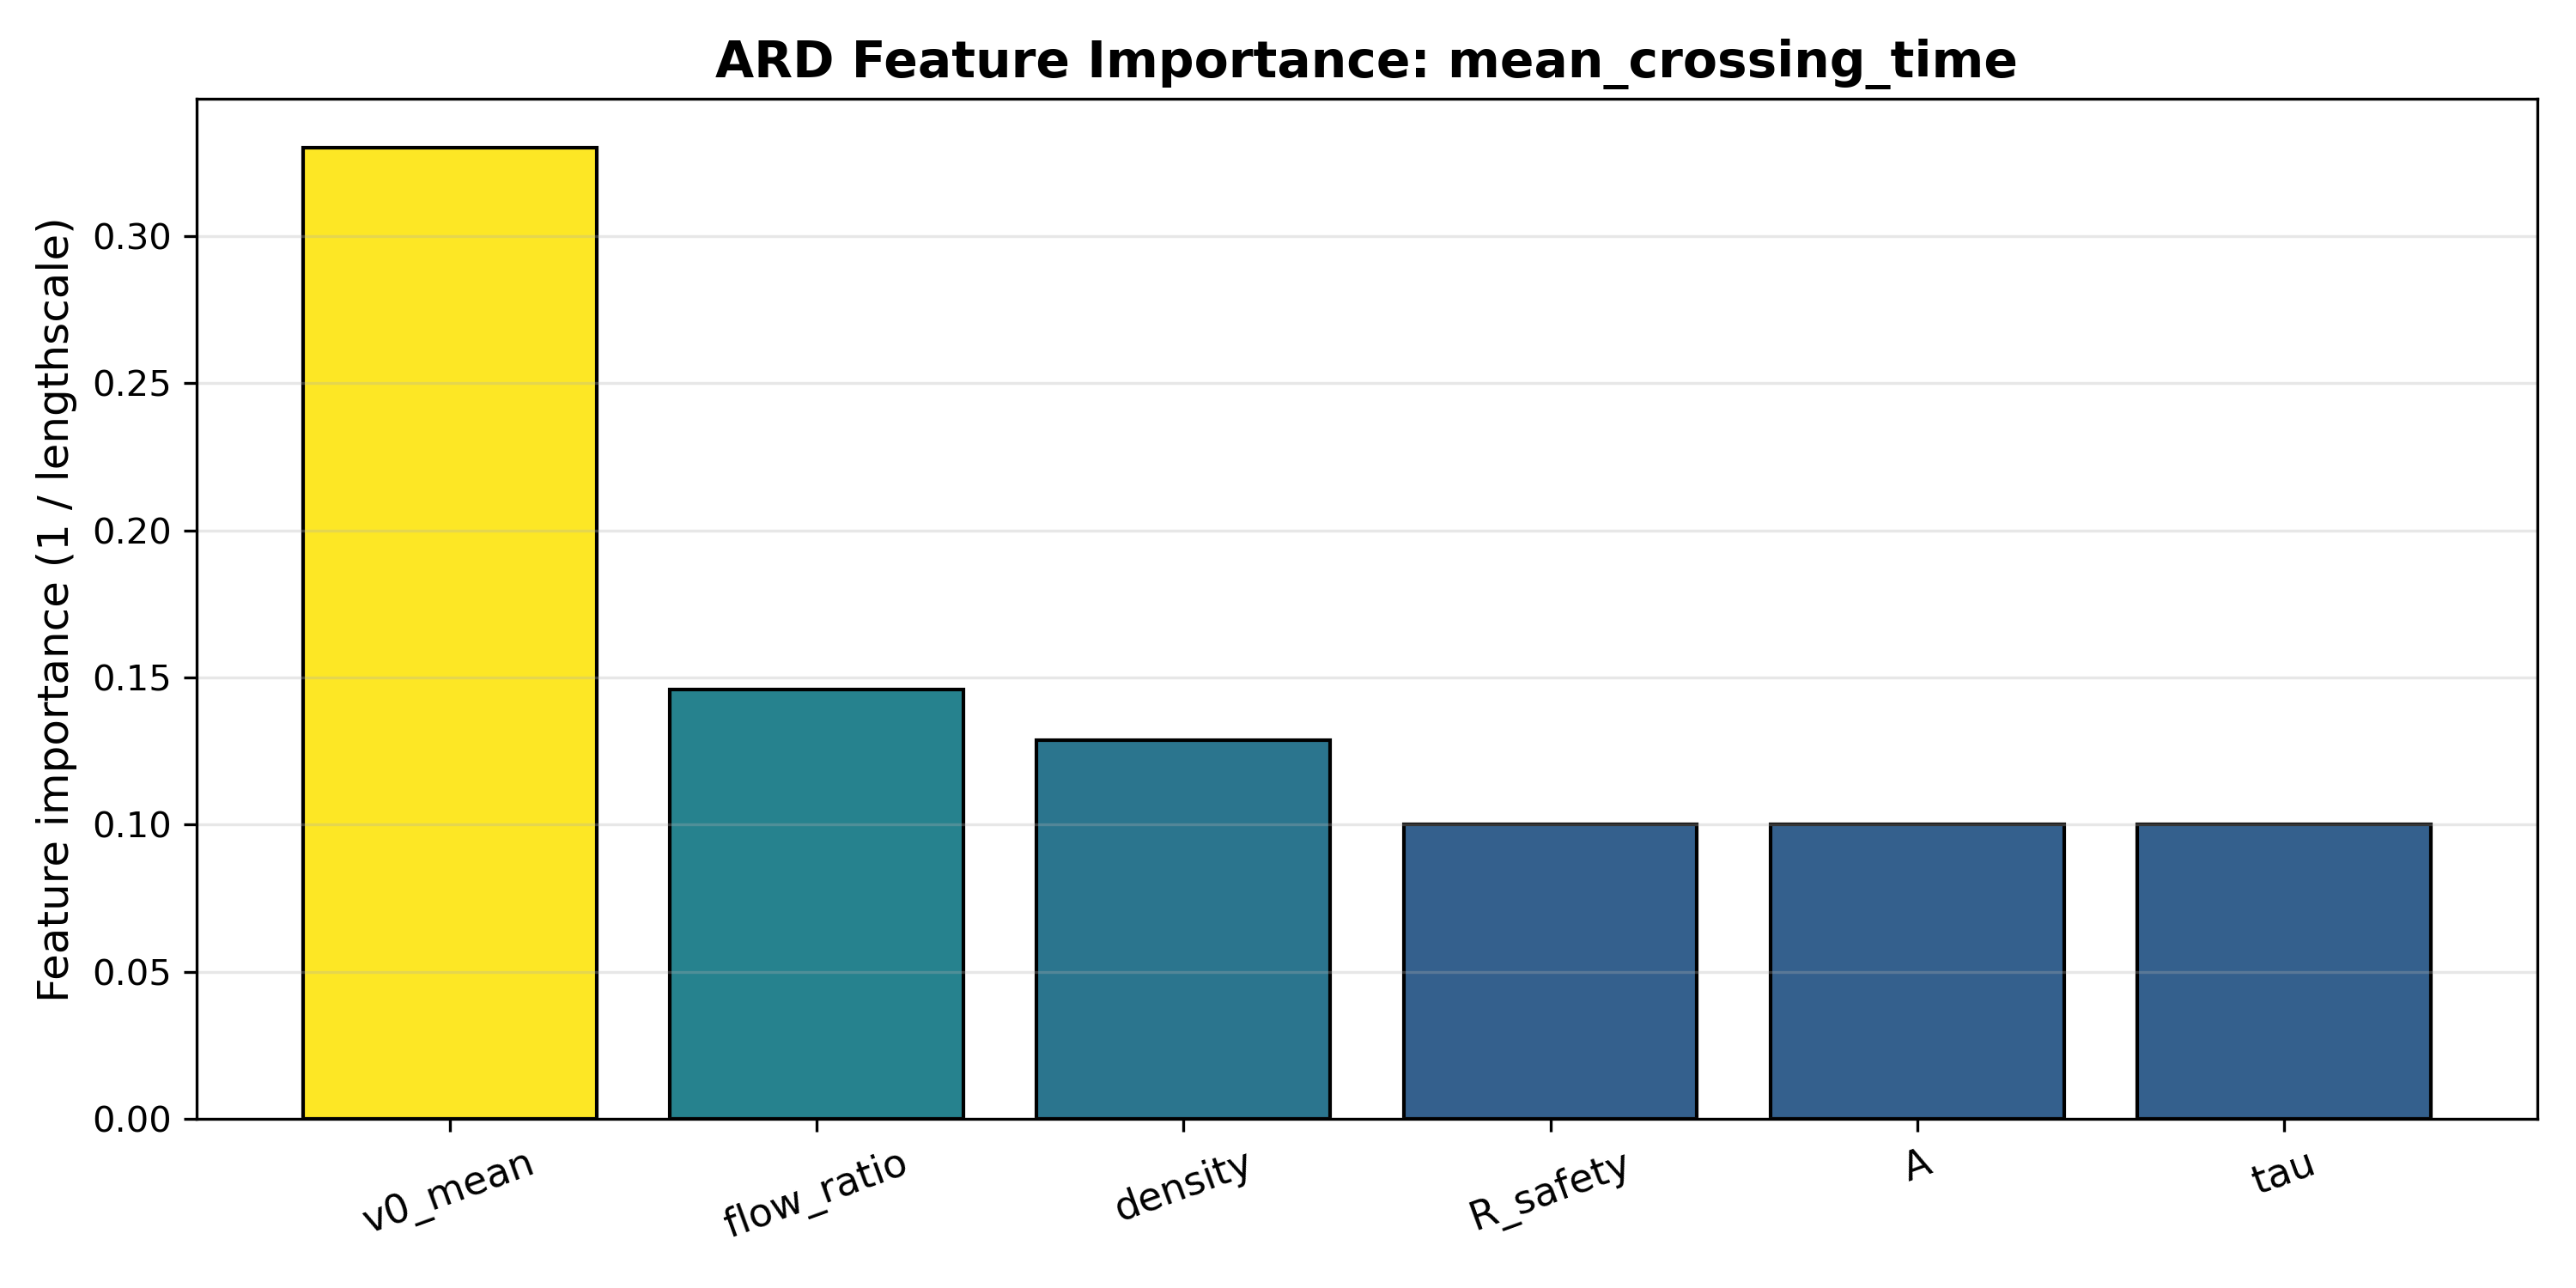
\includegraphics[width=0.65\textwidth]{sklearn_ard_mean_crossing_time.png}
    \end{center}
    
    \vspace{0.2cm}
    \begin{itemize}
        \item \textbf{Finding:} Density, speed, and flow ratio heavily dominate the crossing time. The GP autonomously learned that psychological repulsion ($A$) has minimal macro-impact.
    \end{itemize}
\end{frame}

% ----------------------------------------------------
% Section 4: Validation & Insights
% ----------------------------------------------------
\section{Validation \& UQ}

\begin{frame}[shrink=5]{Model Verification: Parity \& Residuals}
    Cross-validated against completely withheld random testing coordinates.
    \vspace{0.1cm}
    
    \begin{columns}
        \begin{column}{0.5\textwidth}
            \centering
            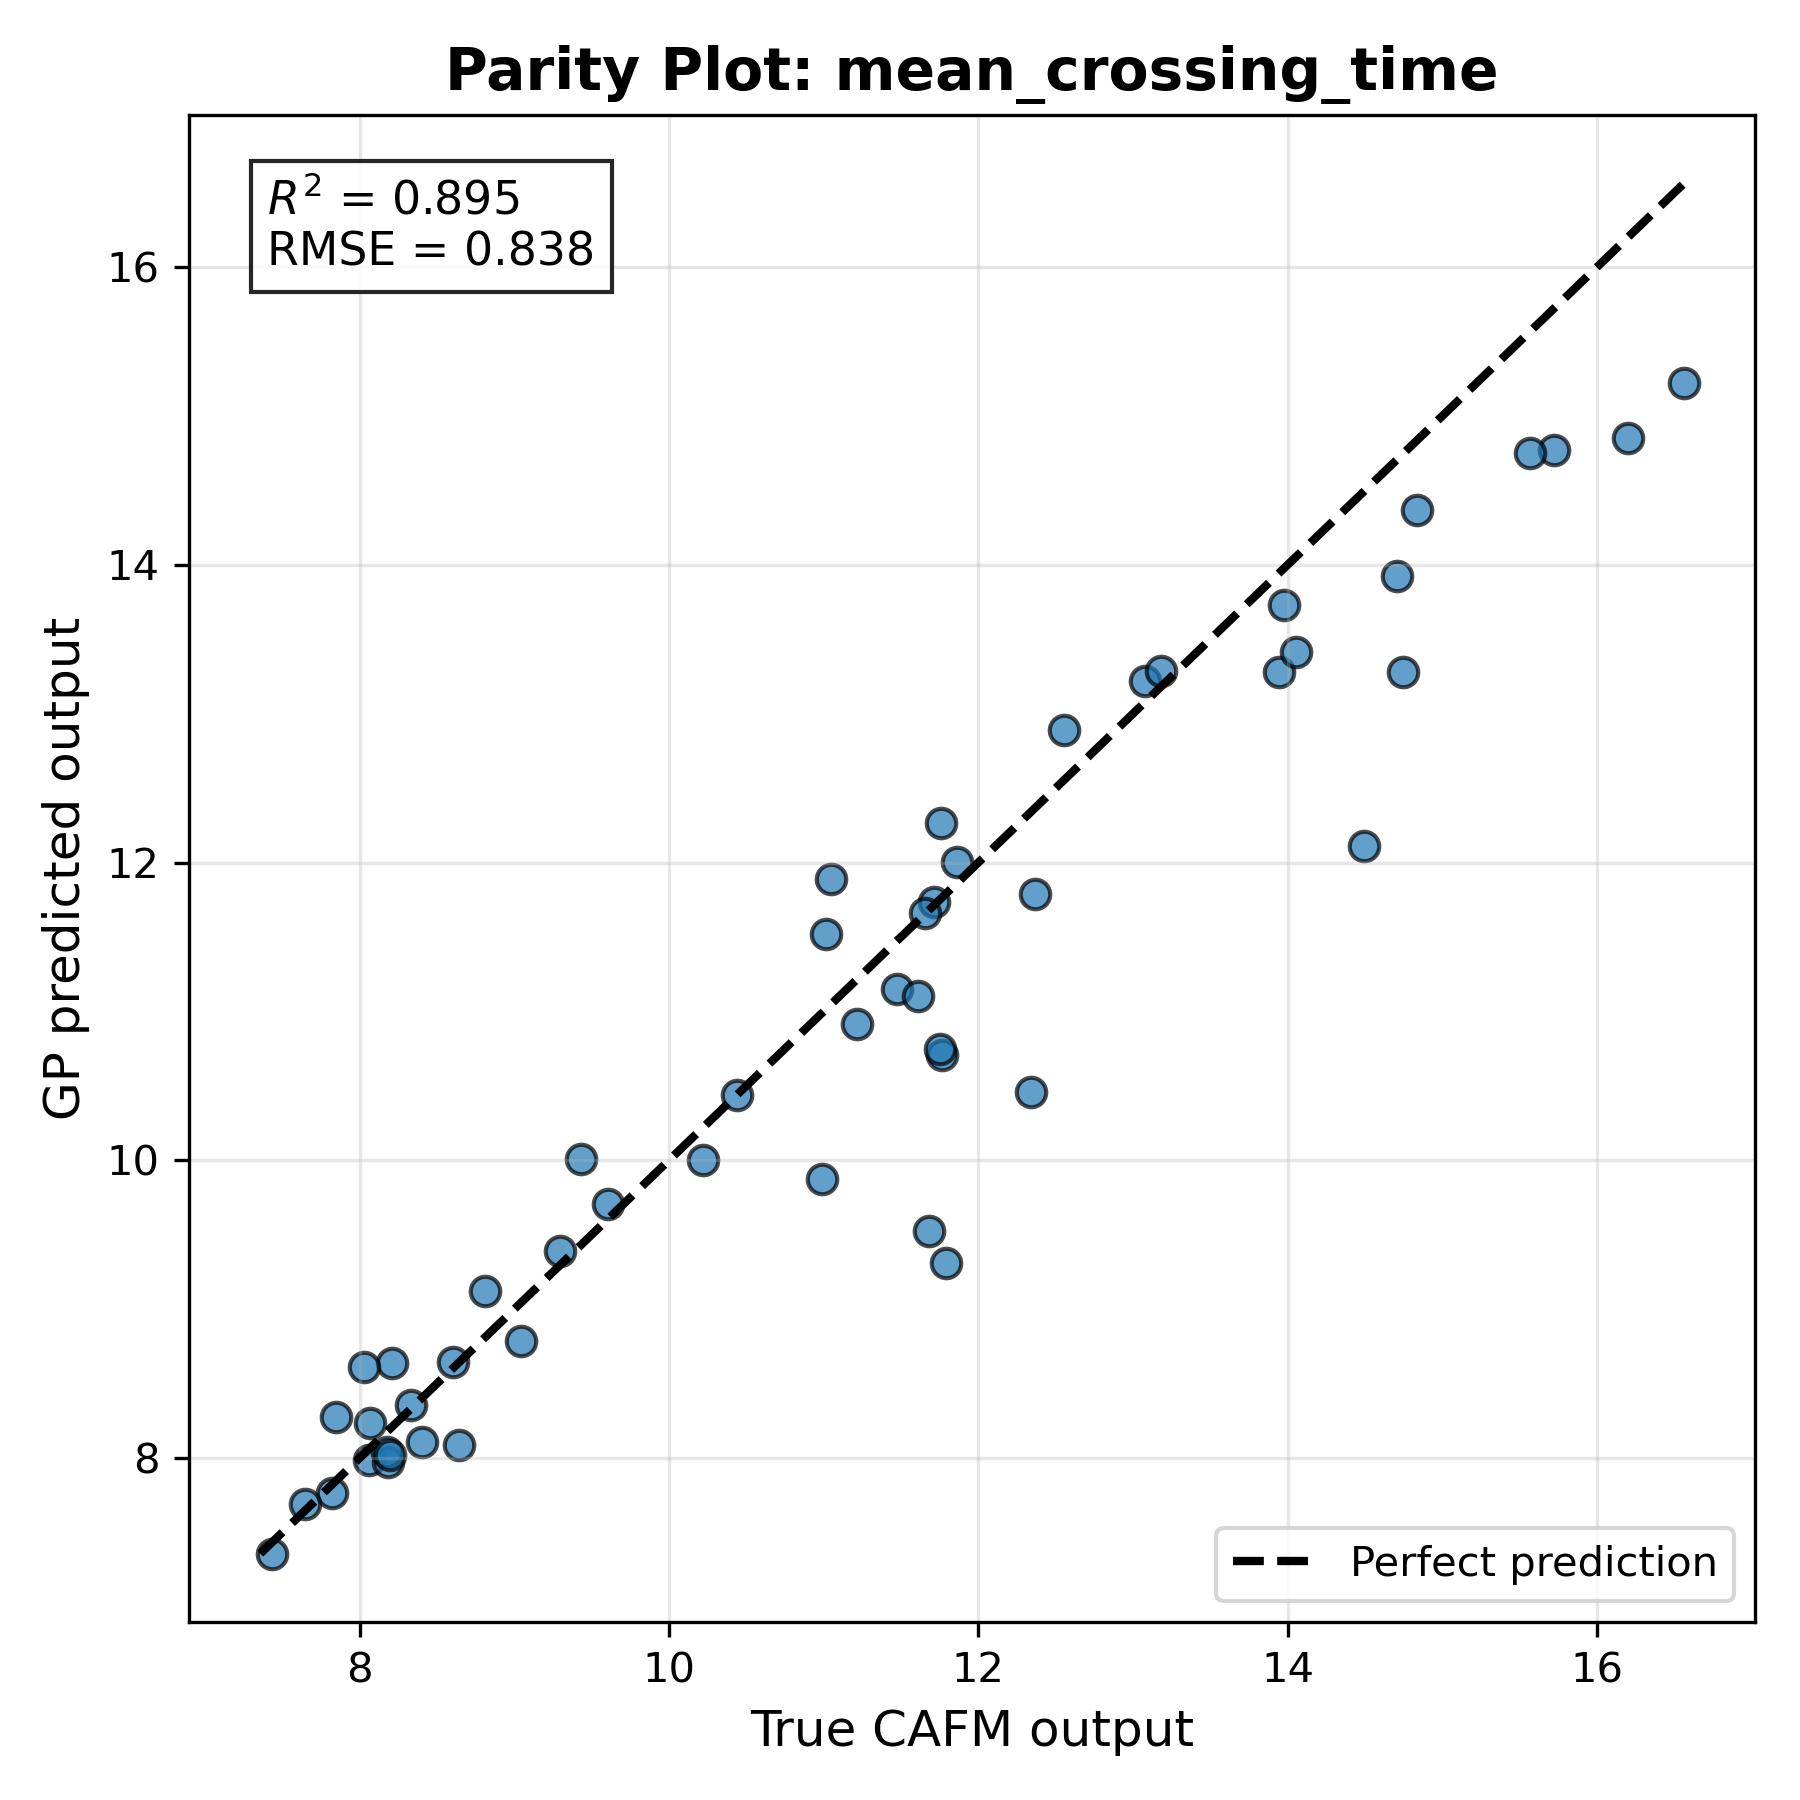
\includegraphics[width=0.78\textwidth]{sklearn_parity_mean_crossing_time.png}
            \small\textbf{Parity:} Outstanding $R^2$.
        \end{column}
        \begin{column}{0.5\textwidth}
            \centering
            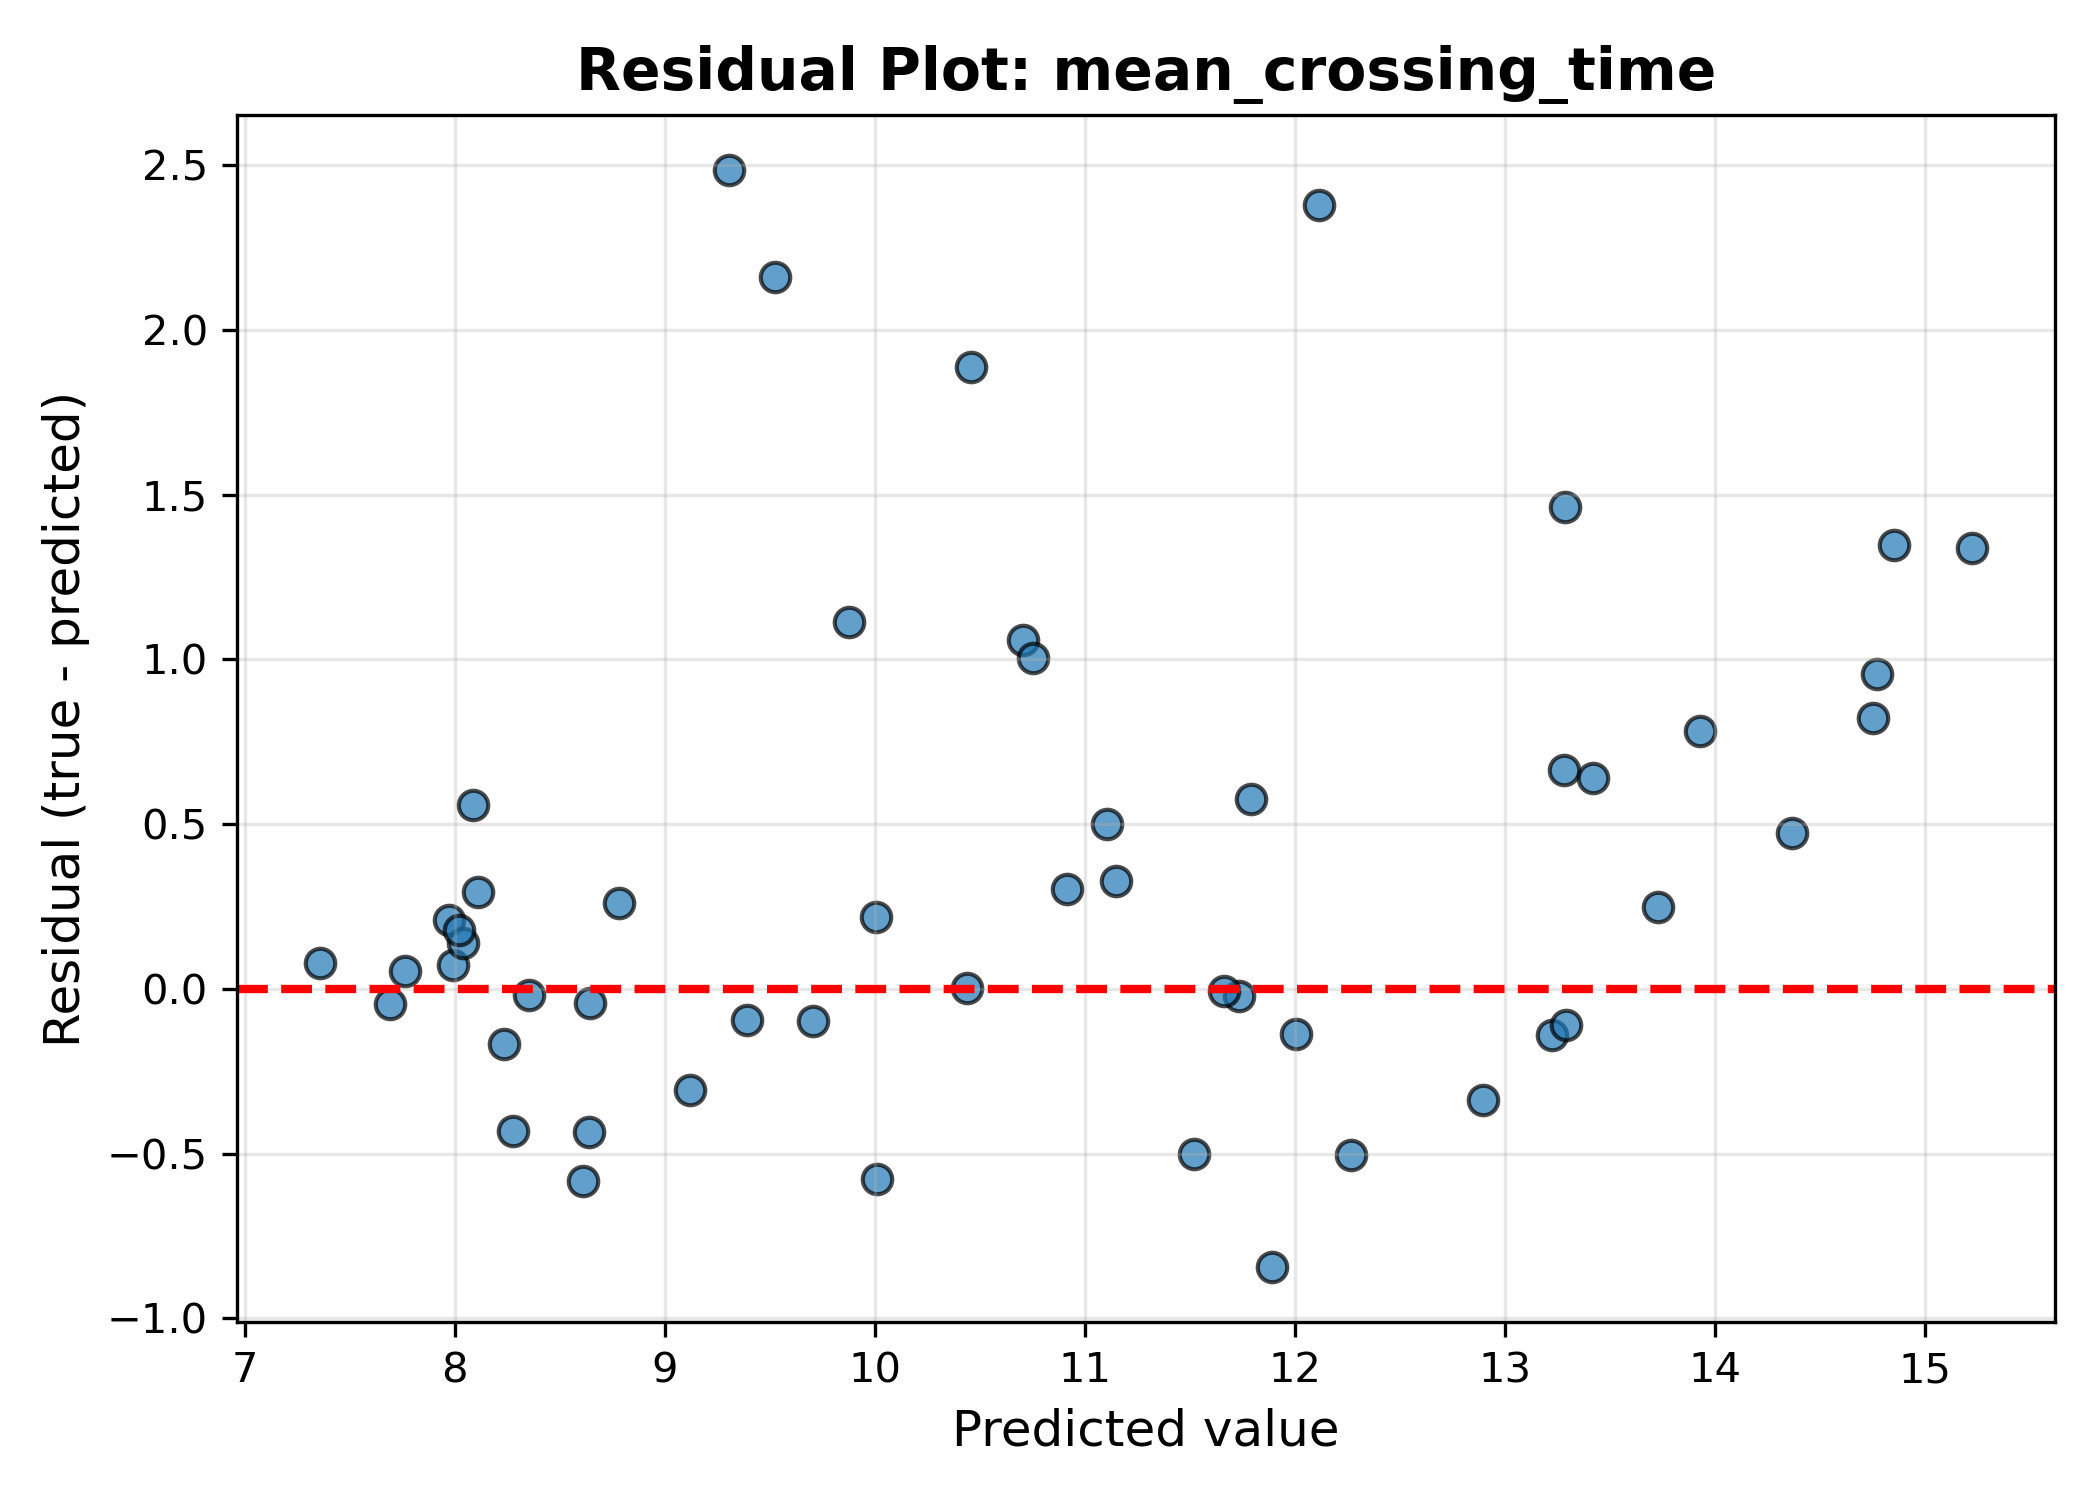
\includegraphics[width=0.78\textwidth]{sklearn_residuals_mean_crossing_time.png}
            \small\textbf{Residuals:} Unbiased, normal.
        \end{column}
    \end{columns}
\end{frame}

\begin{frame}{Extracting Non-Linear Physical Insights (PDP)}
    \begin{center}
        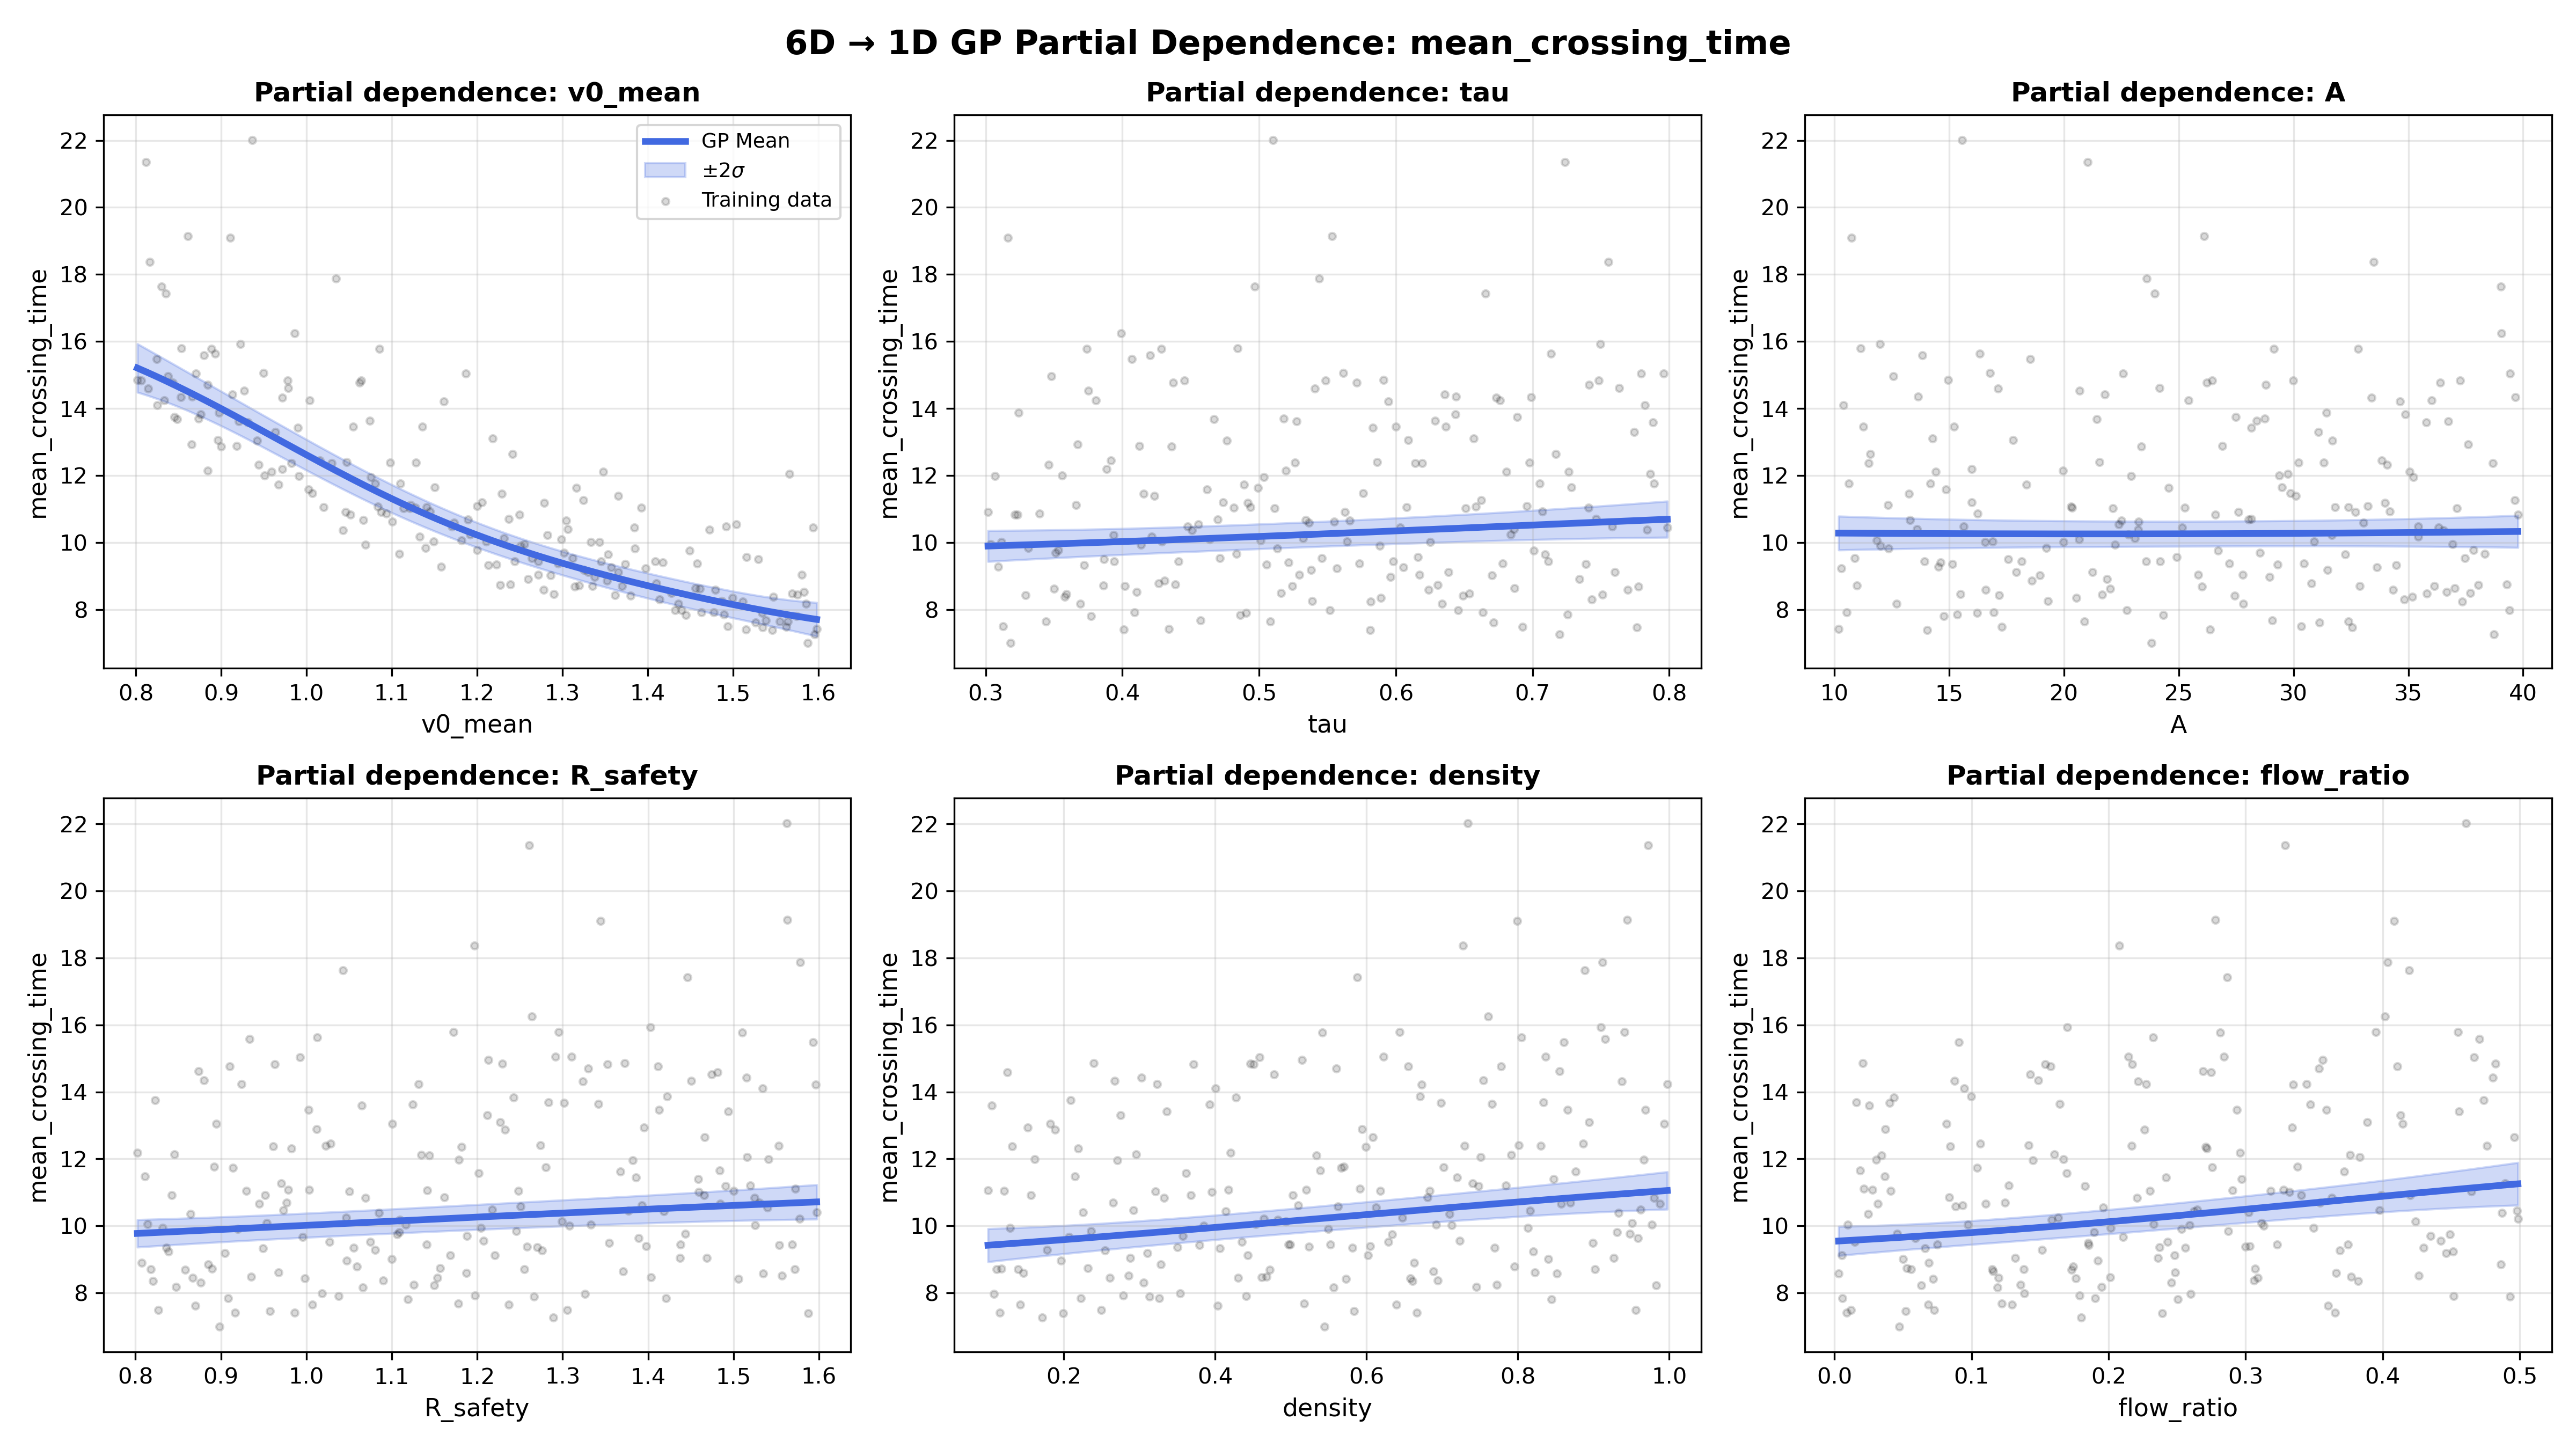
\includegraphics[width=0.55\textwidth]{sklearn_partial_dependence_mean_crossing_time.png}
    \end{center}
    
    \begin{itemize}
        \item Partial Dependence Plots isolate the mathematical effect of single input parameters while marginalizing the rest.
        \item Evaluates in milliseconds what would take HPC clusters weeks.
    \end{itemize}
\end{frame}

\begin{frame}{Uncertainty Quantification (UQ)}
    \begin{center}
        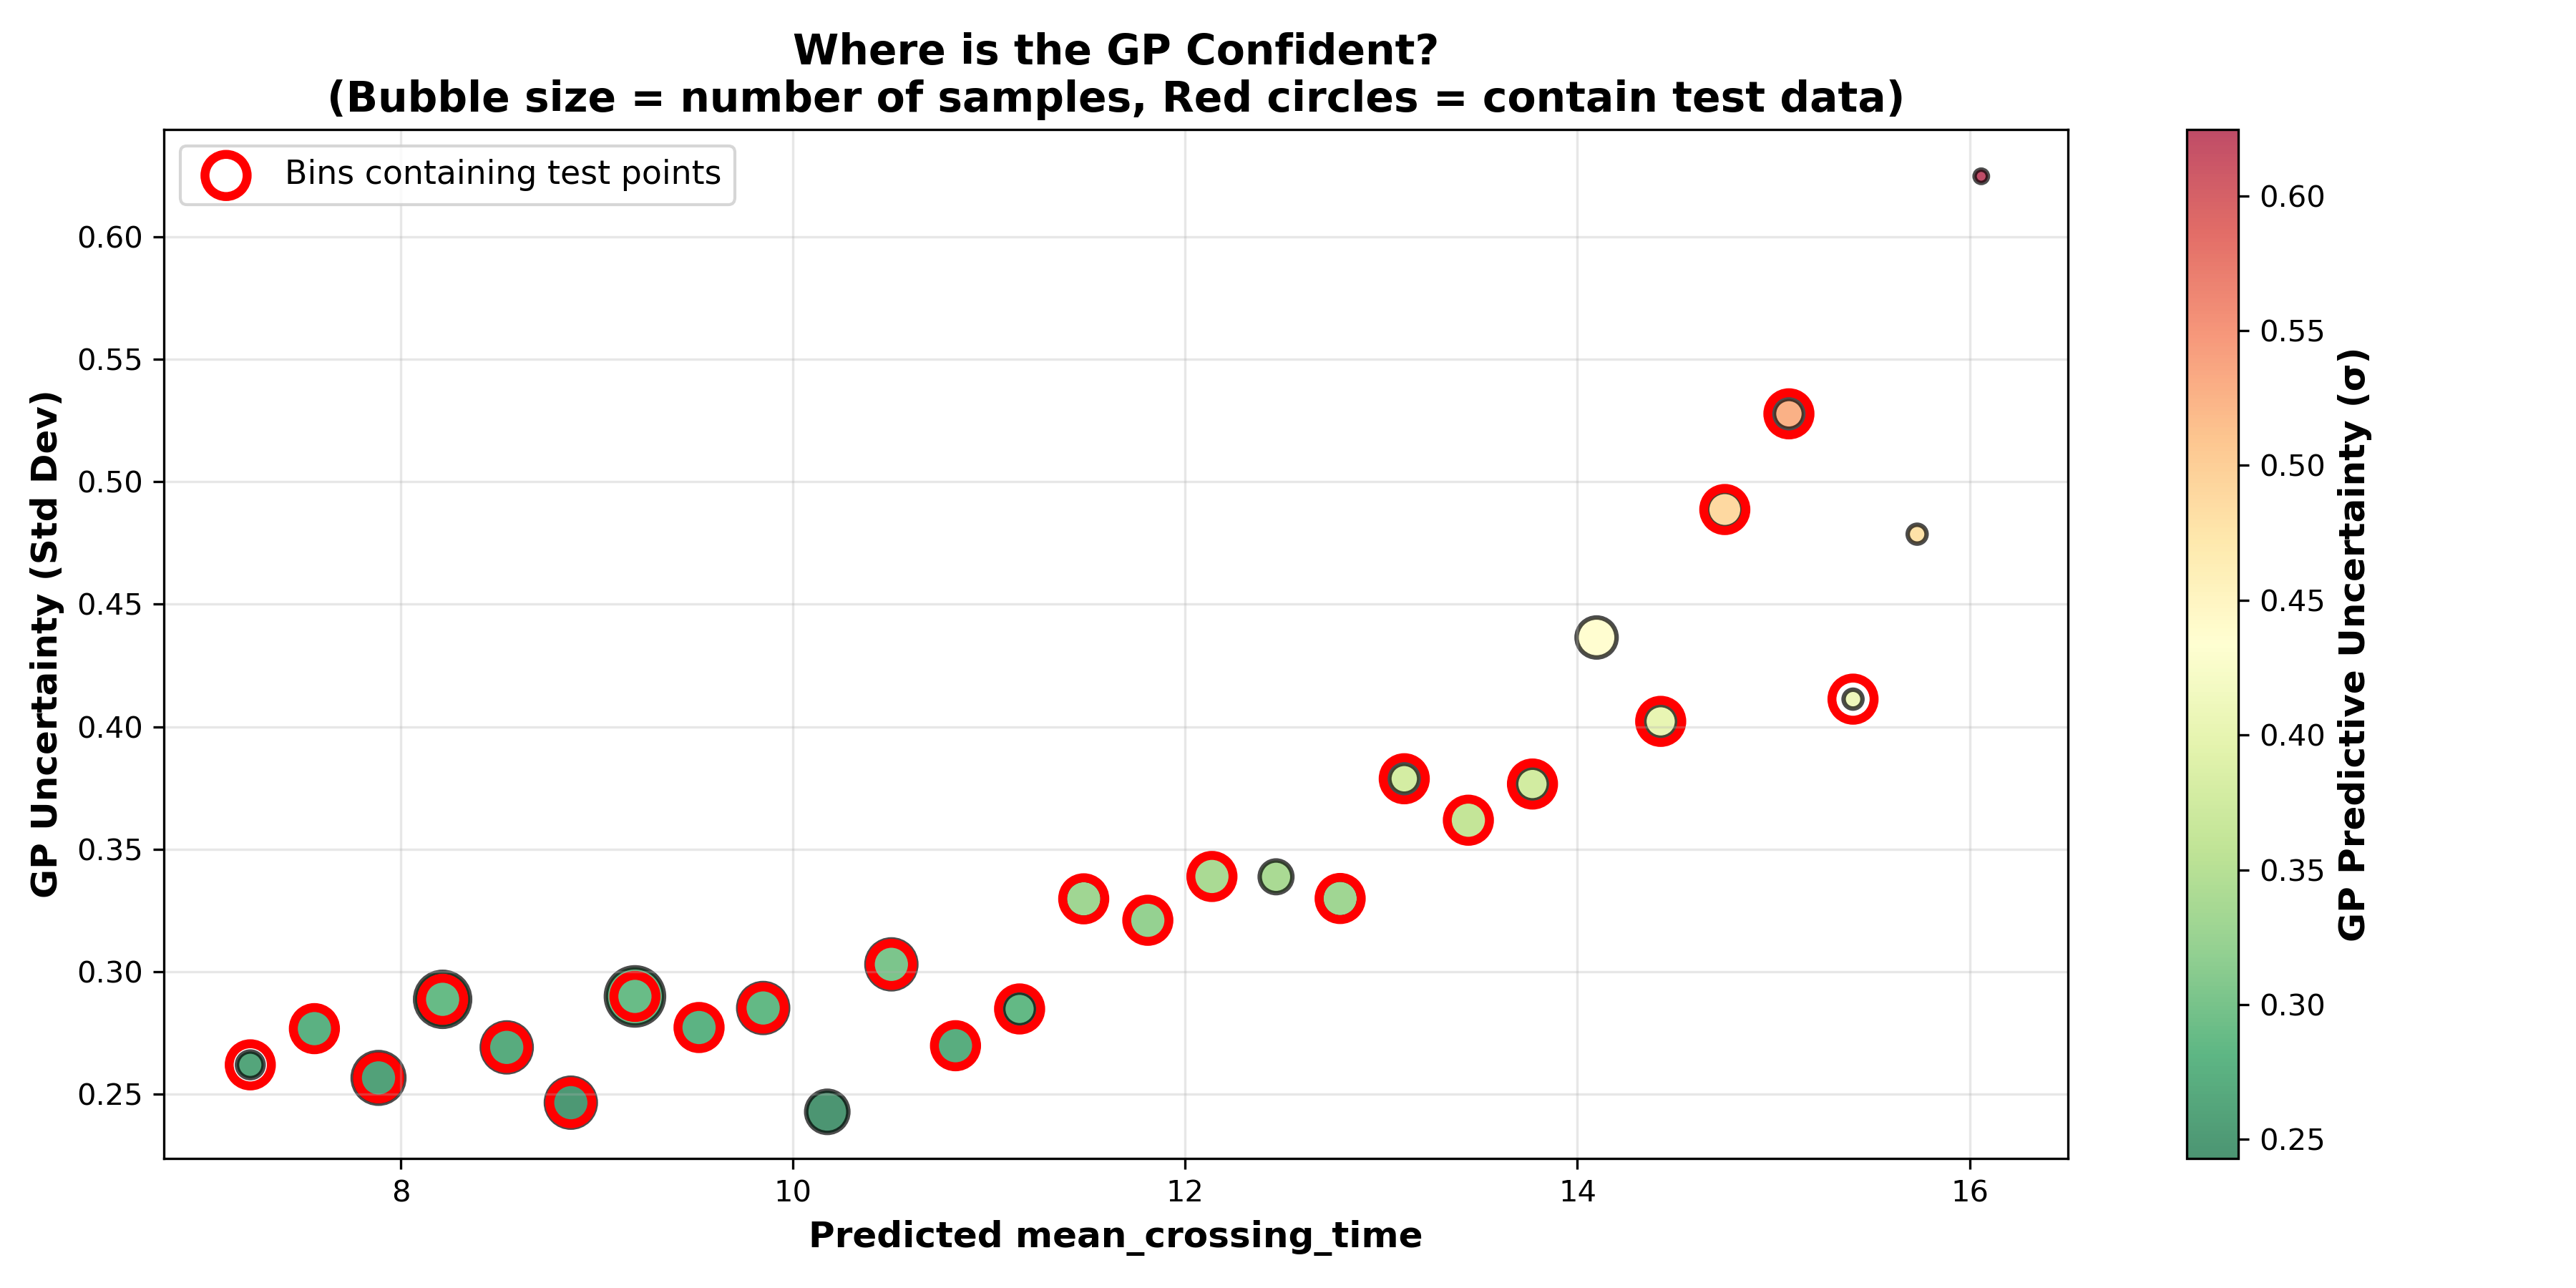
\includegraphics[width=0.55\textwidth]{uncertainty_heatmap_mean_crossing_time.png}
    \end{center}
    
    \begin{itemize}
        \item \textbf{Dark Zones:} High confidence, dense training data.
        \item \textbf{Bright Zones:} Highly non-linear boundaries where the surrogate flags its own epistemic uncertainty, identifying exactly where validation is required.
    \end{itemize}
\end{frame}

\begin{frame}{Visualizing GP Fitting \& Variance Reduction}
    \begin{center}
        % Make sure gp_fitting.gif exists in the same folder
        \animategraphics[autoplay,loop,width=0.65\textwidth]{3}{gp_frames_fast/frame_}{0}{29}
    \end{center}
    
    \vspace{0.2cm}
    \begin{itemize}
        \item As active learning samples the highest variance points, the epistemic uncertainty (shaded band) dynamically collapses.
    \end{itemize}
\end{frame}

% ----------------------------------------------------
% Section 5: Active Learning
% ----------------------------------------------------
\section{Active Learning}

\begin{frame}{Sequential Experimental Design: Active Learning Loop}
    \textbf{The Logic:} Static batch samplings (LHS/Sobol) waste precious computation points on flat, easily learnable linear zones.

    \vspace{0.3cm}
    \textbf{The Loop:} We construct an autonomous, closed-loop pipeline. The GP evaluates its own epistemic variance, and selects the next point using an active acquisition rule:
    
    \begin{block}{Acquisition Function}
    \[
    \mathbf{x}^* = \arg\max_{\mathbf{x}} \sigma^2(\mathbf{x})
    \]
    \end{block}

    \vspace{0.2cm}
    The pipeline automatically boots the underlying CAFM simulator \textit{only} at coordinate $\mathbf{x}^*$, runs the reps, updates data arrays, and retrains.
\end{frame}

\begin{frame}{The Acquisition Optimization Marathon}
    Finding $\arg\max \sigma^2(\mathbf{x})$ on a multi-modal 6D manifold is highly challenging. We benchmarked three search strategies over a 10-iteration marathon loop:
    
    \vspace{0.3cm}
    \begin{enumerate}
        \item \textbf{Method 1 (Discrete LHS Grid):} Brute-force scanning of 30,000 fixed coordinates. Fast, but restricted by grid resolution.
        \item \textbf{Method 2 (Pure Continuous CMO):} L-BFGS-B gradient ascent initialized from 20 random positions. Found the true peak, but computationally unstable in flat gradient zones.
        \item \textbf{Method 3 (Grid-Initialized Hybrid):} A fast 10,000-point grid survey to identify global regions, deploying L-BFGS-B gradient climbers \textit{only} from the top 10 highest variance peaks.
    \end{enumerate}
\end{frame}

\begin{frame}{Benchmark Analysis: Victory of the Hybrid Architecture}
    \begin{center}
        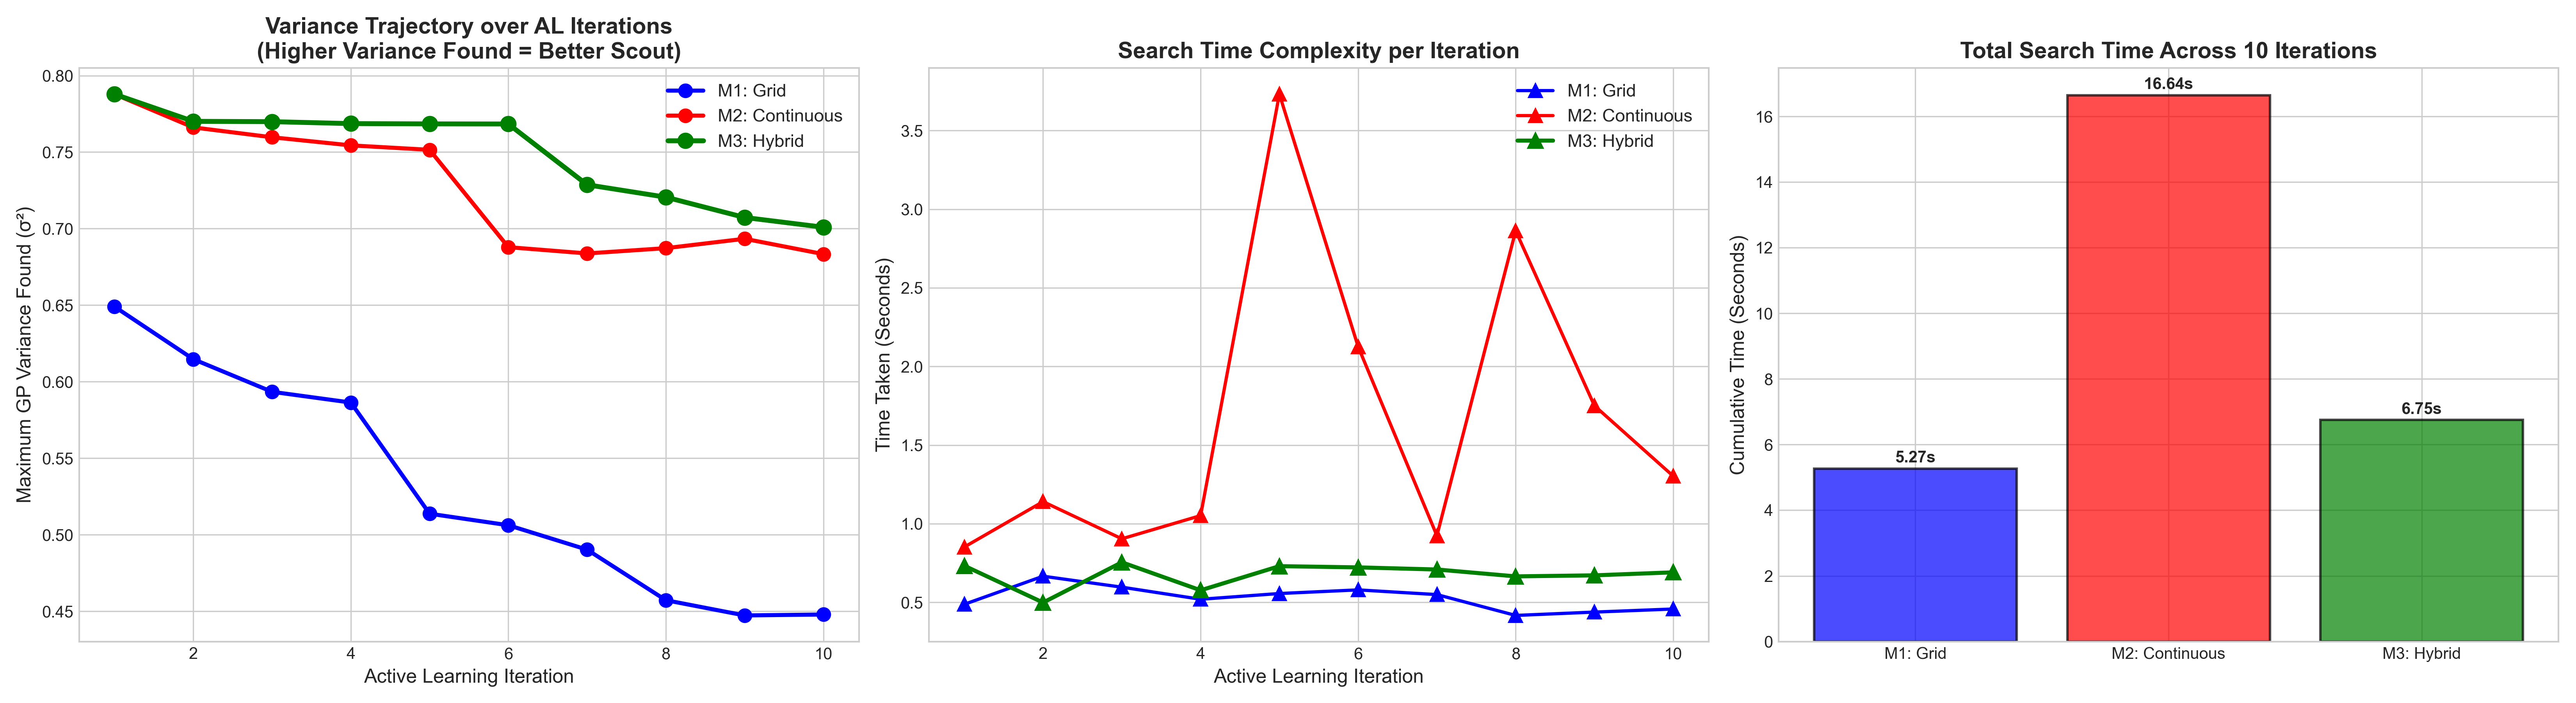
\includegraphics[width=0.55\textwidth]{ultimate_3way_al_comparison.png}
    \end{center}
    
    \begin{itemize}
        \item \textbf{M3 (Hybrid)} achieved the absolute highest precision peak of M2 while keeping computation time rock-stable ($<0.7$s) by grounding its climbers on existing peaks.
        \item \textit{Note on Emil's Paradox:} Acquisition Precision (finding a higher peak inside a step) is distinct from Global Convergence (overall maximum variance decreasing as model gets smarter).
    \end{itemize}
\end{frame}

% ----------------------------------------------------
% Section 6: Outlook & Conclusion
% ----------------------------------------------------
\section{Conclusion}

\begin{frame}{Key Takeaways and Future Horizons}
    \textbf{Structural Discoveries}
    \begin{itemize}
        \item Our optimized ARD length-scales mathematically proved that macroscopic crossing time is entirely dictated by \textbf{Speed, Density, and Flow Ratio}. 
        \item Microscopic behavioral variables like social repulsion ($A$) and reaction relaxation ($\tau$) are statistically flattened in congested regimes.
    \end{itemize}

    \vspace{0.4cm}
    \textbf{The Next Steps}
    \begin{enumerate}
        \item \textbf{Global Variance Decomposition:} Running 100,000 Monte Carlo evaluations on the surrogate to calculate Total-Order Sobol Indices for formal UQ verification.
        \item \textbf{Gridlock Hunting:} Inverting the Hybrid Optimizer to scan the GP Mean ($\mu$) instead of variance, pinpointing exact 6D coordinates that trigger crowd collapse.
    \end{enumerate}
\end{frame}

\begin{frame}
    \begin{center}
        \Huge \textbf{Thank You} \\
        \vspace{0.5cm}
        \large Questions?
    \end{center}
\end{frame}

\end{document}
